\documentclass[11pt]{article}
\usepackage[a4paper,margin=1in]{geometry}
\usepackage{amsmath,amssymb,amsthm,bm}
\usepackage{graphicx,booktabs,multirow,xcolor}
\usepackage{algorithm,algpseudocode}
\usepackage[numbers,sort&compress]{natbib}
\usepackage[colorlinks=true,linkcolor=blue!50!black,citecolor=blue!50!black,urlcolor=blue!50!black]{hyperref}
\usepackage{caption}\captionsetup{font=small}
\newtheorem{proposition}{Proposition}
\newtheorem{assumption}{Assumption}
\newcommand{\E}{\mathbb{E}}
\newcommand{\Acc}{\mathrm{Acc}}
\newcommand{\oob}{\mathrm{OOB}}

\title{Free Reference Sets: Label-Free Accuracy Estimation under Distribution Shift for Bagged Ensembles via Size-Extrapolated Out-of-Bag Scores}
\author{Siddhant Agarwal\\ Independent Researcher\\ ORCID: \href{https://orcid.org/0009-0004-7658-2091}{0009-0004-7658-2091}}
\date{}

\begin{document}
\maketitle

\begin{abstract}
Estimating the accuracy of a deployed classifier on unlabeled, distribution-shifted data is central to model monitoring. Existing estimators, including average thresholded confidence, difference of confidences, importance-weighted validation and recent tabular methods, all require a labeled reference set held out from training. This forces a trade-off between model quality and estimate reliability. We show that for bagged ensembles such as random forests the trade-off is unnecessary: out-of-bag (OOB) predictions provide a free reference set covering the whole training sample. We prove that an OOB prediction is an exact held-out prediction of a \emph{smaller} ensemble of about $T/e$ members, and that the resulting mismatch biases naive OOB plug-ins by $O(1/T)$. We remove this bias with size-matched estimation extrapolated in $1/m$, add randomized tie-breaking for the discrete confidences of tree ensembles, and obtain cross-fitted importance weights from an OOB domain classifier. We evaluate the approach in a pre-registered study of 5{,}212 estimation tasks: 40 synthetic task families, all 72 datasets of the OpenML-CC18 benchmark, four shift types, ensemble- and sample-size sweeps, and both random forests and Extra-Trees. The OOB route lowered absolute estimation error relative to the holdout route in all 24 planned comparisons, by 5--40\%. On the 72 real datasets the reductions were 5--21\%, significant at the dataset level for every estimator family, and importance weighting improved on 66 of 72 datasets. The deployed model was simultaneously 0.35--1.73 percentage points more accurate. Gains were largest for small datasets, in-distribution and under covariate shift, and vanished for some estimators under corruption shift. We also report where our hypotheses failed. Size extrapolation consistently helps threshold-based estimators but not plain and importance-weighted ones under shift, no estimator family dominates across shift types, and a large improvement in detecting harmful shift seen on synthetic data did not replicate on real data.

\end{abstract}

\noindent\textbf{Keywords:} distribution shift; performance estimation without labels; random forests; out-of-bag estimation; model monitoring; importance weighting

\section{Introduction}
\label{sec:intro}

A model deployed in the field is almost never evaluated on data drawn from its training distribution. Covariates drift, sub-populations change, sensors degrade, and class priors move \citep{rabanser2019failing}. Ground-truth labels for the deployment data, however, typically arrive late, are expensive, or never arrive at all. This has motivated a growing literature on \emph{label-free accuracy estimation}: predicting the accuracy of a fixed classifier on an unlabeled target sample. Representative methods include the difference of confidences (DoC) \citep{guillory2021doc}, average thresholded confidence (ATC) \citep{garg2022atc}, importance-weighted validation \citep{sugiyama2007iwcv}, model disagreement \citep{jiang2022gde,baek2022aotl}, and, for tabular data, the recent probabilistic adaptive performance estimation (PAPE) \citep{bialek2025pape}.

Almost all of these methods share a requirement that is easy to overlook: a \emph{labeled reference set} drawn from the source distribution and \emph{not used for training}. ATC learns its threshold on it, DoC subtracts its confidence, importance weighting averages its losses, and PAPE fits its calibrator on it. In practice the reference set is carved out of the training data, which creates a dilemma. A large reference set makes the estimate reliable but makes the deployed model worse. A small reference set keeps the model strong but makes the estimate noisy. The dilemma is sharpest exactly where it matters most: small or medium tabular datasets, in which tree ensembles remain the method of choice \citep{grinsztajn2022tabular}.

This paper observes that, for bagged ensembles such as random forests \citep{breiman2001rf}, the dilemma is avoidable. Each training point is left out of roughly $e^{-1}\approx 37\%$ of the bootstrap samples, so the out-of-bag (OOB) prediction for every training point is a genuine held-out prediction \citep{breiman1996oob}. The entire training set can therefore serve as a labeled reference set \emph{at no cost}, and the deployed model can be trained on all available data. OOB predictions are routinely used to estimate in-distribution error, but to our knowledge they have not been used as the reference sample for estimating accuracy under distribution shift.

Plugging OOB predictions into existing estimators is not quite enough, however. We show that an OOB prediction is a valid held-out prediction of a \emph{different}, smaller model: a sub-ensemble of $\approx T/e$ trees, not the $T$-tree ensemble that is actually deployed (Proposition~\ref{prop:oob}). Both the accuracy and the confidence distribution of a sub-ensemble differ systematically from those of the full ensemble, so the naive plug-in is biased. The bias is large for small ensembles and vanishes as $T\to\infty$. We remove it with \emph{size-matched extrapolation}. Each estimator is recomputed with source and target scores produced by ensembles of identical size $m$, over a grid of sizes. The resulting curve is then extrapolated to $m=T$ using the known $O(1/m)$ convergence of randomized ensembles \citep{ng2001voting,lopes2016sharp,cannings2017rp,lopes2019aos}. We also identify a practical pitfall: tree-vote confidences are discrete, so threshold-based estimators such as ATC need randomized tie-breaking.

\paragraph{Contributions.}
\begin{enumerate}
\item We formalize the OOB sample of a bagged ensemble as a \emph{free reference set} for label-free accuracy estimation under shift. We characterize precisely which model it is a held-out sample for (Proposition~\ref{prop:oob}).
\item We propose size-matched, $1/m$-extrapolated OOB versions of four estimator families (plain, DoC, ATC, importance weighting). We also propose an OOB domain classifier that yields cross-fitted density ratios without data splitting.
\item We report a pre-registered empirical study with 5{,}212 estimation tasks. It covers 40 synthetic task families, all 72 real datasets of the OpenML-CC18 benchmark suite \citep{bischl2021openml} plus three small real datasets, four shift types at several severities, and sweeps over ensemble size and sample size, for random forests and Extra-Trees.
\item We report, including where our hypotheses were refuted, when each component helps. The free reference set gives statistically robust gains on synthetic and real data, largest for small datasets and smallest under corruption shift. Extrapolation matters mainly for small ensembles and for threshold-based estimators.
\end{enumerate}

\section{Related work}
\label{sec:related}

\paragraph{Label-free accuracy estimation.}
Confidence-based estimators predict target accuracy from the model's scores on unlabeled target data. Average confidence (AC) is the simplest and requires perfect calibration. DoC \citep{guillory2021doc} corrects AC by the gap between source and target confidence. ATC \citep{garg2022atc} learns a confidence threshold on labeled source data and reports the fraction of target points above it. Disagreement-based methods \citep{jiang2022gde,baek2022aotl,kirsch2022note} relate the agreement of independently trained models to their accuracy. Regression-on-features methods train a meta-model across many shifted datasets \citep{deng2021labels}. Mandoline \citep{chen2021mandoline} uses user-specified slicing functions for importance reweighting. For tabular data, \citet{bialek2025pape} recently proposed PAPE, which combines density-ratio estimation with calibration on a labeled reference set. They benchmarked it against ATC, DoC, confidence-based performance estimation and importance weighting on 959 dataset--model pairs derived from US census data \citep{ding2021folktables}. Every one of these methods needs a labeled reference set or a collection of labeled shifted datasets; our contribution is orthogonal and makes the reference set free for bagged models.

\paragraph{Covariate shift and importance weighting.}
Under covariate shift, $p(y\mid x)$ is invariant, and the target risk can be estimated by reweighting source losses with the density ratio $w(x)=q(x)/p(x)$ \citep{shimodaira2000,sugiyama2007iwcv}. The ratio is commonly estimated with a probabilistic domain classifier \citep{rabanser2019failing}. Under label shift, $p(x\mid y)$ is invariant instead \citep{lipton2018bbse}. Under support shift, such as corruptions \citep{hendrycks2019corruptions}, neither assumption holds.

\paragraph{Out-of-bag estimation and randomized ensembles.}
OOB estimation dates to \citet{breiman1996oob} and \citet{breiman2001rf}. It has been used for variance estimation \citep{wager2014ij} and for conformal prediction via the jackknife+-after-bootstrap \citep{kim2020jab}, always for in-distribution guarantees. The convergence of a randomized ensemble's error to its infinite-ensemble limit has been studied by \citet{ng2001voting}, \citet{lopes2016sharp}, \citet{cannings2017rp} and \citet{lopes2019aos}. These works show that the expected excess error decays at the fast rate $1/t$ in the number of members under various conditions. We exploit this rate for Richardson-type extrapolation \citep{richardson1911} of shift-aware estimators.

\section{Problem setup}
\label{sec:setup}

Let $P$ and $Q$ be source and target distributions on $\mathcal X\times\{1,\dots,K\}$. We observe a labeled source sample $S=\{(x_i,y_i)\}_{i=1}^n\sim P^n$ and an unlabeled target sample $X^Q=\{\tilde x_j\}_{j=1}^{n_Q}\sim Q_X^{n_Q}$. A bagged ensemble consists of $T$ base learners $h_1,\dots,h_T$. Learner $h_t$ is trained on a bootstrap multiset $B_t$ of $n$ draws from $S$, with internal randomness $\theta_t$, and outputs a probability vector $h_t(x)\in\Delta^{K-1}$. For an index set $U\subseteq\{1,\dots,T\}$ we write $\bar h_U(x)=|U|^{-1}\sum_{t\in U}h_t(x)$, $f_U(x)=\arg\max_k \bar h_{U,k}(x)$ and $c_U(x)=\max_k\bar h_{U,k}(x)$ (the confidence). The deployed model is $f_{[T]}$. The estimand is its target accuracy,
\begin{equation}
\Acc_Q(f_{[T]})=\Pr_{(x,y)\sim Q}\big[f_{[T]}(x)=y\big].
\end{equation}
A \emph{reference-set estimator} $\Phi$ maps labeled reference scores $\{(c(x_i),\mathbb 1[f(x_i)=y_i])\}$ and unlabeled target scores $\{c(\tilde x_j)\}$ (and possibly the covariates themselves) to an accuracy estimate. We consider four families:
\begin{align*}
\text{plain:}\quad &\hat a=\textstyle\frac1{n_r}\sum_i \mathbb 1[f(x_i)=y_i],\\
\text{DoC:}\quad &\hat a-\big(\overline{c(x_i)}-\overline{c(\tilde x_j)}\big),\\
\text{ATC:}\quad &\textstyle\frac1{n_Q}\sum_j \mathbb 1[c(\tilde x_j)>\tau],\ \ \tau:\ \tfrac1{n_r}\textstyle\sum_i \mathbb 1[c(x_i)>\tau]=\hat a,\\
\text{IW:}\quad &\textstyle\sum_i \hat w(x_i)\,\mathbb 1[f(x_i)=y_i]\big/\sum_i\hat w(x_i),
\end{align*}
where $\hat w$ estimates $q(x)/p(x)$. The standard \emph{holdout} route (HO) trains the ensemble on a fraction $1-\rho$ of $S$ and uses the remaining $\rho n$ points as the reference set. Its estimand is the accuracy of that smaller-data model.

\section{Method}
\label{sec:method}

\subsection{The OOB sample is a free reference set, for a smaller model}

Let $O_i=\{t: i\notin B_t\}$ be the set of learners for which point $i$ is out of bag, and let $f^{\oob}(x_i)=f_{O_i}(x_i)$.

\begin{proposition}[What OOB scores are a held-out sample of]
\label{prop:oob}
Fix $i$ and condition on $|O_i|=m\ge1$. Then the learners $\{h_t\}_{t\in O_i}$ are i.i.d.\ draws of a learner trained on $n$ uniform draws from $S_{-i}=S\setminus\{(x_i,y_i)\}$, and they are independent of $(x_i,y_i)$ given $S_{-i}$. Consequently, for any bounded function $g$ of the confidence and correctness,
\[
\E\big[g\big(c_{O_i}(x_i),\mathbb 1[f_{O_i}(x_i)=y_i]\big)\,\big|\,|O_i|=m\big]=\E_{(x,y)\sim P}\big[g\big(c_{U_m}(x),\mathbb 1[f_{U_m}(x)=y]\big)\big],
\]
where $U_m$ is an $m$-member ensemble trained on a sample of size $n-1$. Moreover, $|O_i|\sim\mathrm{Bin}(T,(1-1/n)^n)$, whose mean is $\approx T/e$.
\end{proposition}
\begin{proof}[Proof sketch]
Conditional on $i\notin B_t$, each of the $n$ draws that form $B_t$ is uniform on the remaining $n-1$ indices, and the draws are independent across draws and across learners. The learners' internal randomness $\theta_t$ is independent of the data. Hence $\{h_t\}_{t\in O_i}$ depends on $S$ only through $S_{-i}$, and $(x_i,y_i)\sim P$ is a fresh draw relative to them. The binomial law follows because the events $\{i\notin B_t\}$ are independent across $t$, each with probability $(1-1/n)^n$.
\end{proof}

Proposition~\ref{prop:oob} says that the OOB sample is an exact (leave-one-out) reference sample for \emph{an $m$-member ensemble}, with $m$ random and concentrated near $T/e$. Two discrepancies separate it from the deployed model: training-set size $n-1$ versus $n$, which is negligible, and ensemble size $m$ versus $T$, which is not negligible for moderate $T$. The size discrepancy affects reference-set estimators through two channels. First, the reference accuracy $\hat a$ underestimates the full ensemble's accuracy. Second, the reference confidences are systematically lower and more dispersed than the target confidences produced by the full ensemble. Both channels corrupt DoC and ATC. Only the first corrupts plain and IW estimators.

\subsection{Size-matched extrapolation}

To remove the size discrepancy, we evaluate every estimator at a common ensemble size on both sides and extrapolate in $1/m$.

\begin{assumption}[$1/m$ expansion]
\label{ass:rate}
For estimator family $\Phi$, let $\phi(m)=\E[\Phi_m]$, where $\Phi_m$ is computed with source scores from size-$m$ OOB sub-ensembles and target scores from size-$m$ random sub-ensembles. Then $\phi(m)=\phi_\infty+b/m+r(m)$ with $|r(m)|\le C/m^2$.
\end{assumption}
For the plain family, Assumption~\ref{ass:rate} is the fast $1/t$ convergence of the expected error of randomized ensembles established under various conditions in \citep{ng2001voting,lopes2016sharp,cannings2017rp}. For the other families we verify it empirically (Section~\ref{sec:mech}).

\begin{algorithm}[t]
\caption{Size-matched, $1/m$-extrapolated OOB estimation (OOB-$\Phi$-X)}
\label{alg:x}
\begin{algorithmic}[1]
\Require bagged ensemble $\{h_t\}_{t=1}^T$ with OOB sets $\{O_i\}$; labeled source $S$; unlabeled target $X^Q$; estimator family $\Phi$; repetitions $R$; grid size $G$
\State $m_{\max}\gets$ 10th percentile of $\{|O_i|\}$; grid $\mathcal M\gets$ $G$ integers equally spaced in $[m_{\max}/4,\,m_{\max}]$
\For{$m\in\mathcal M$}
  \For{$r=1,\dots,R$}
    \State for each $i$ with $|O_i|\ge m$: draw $U_i\subset O_i$ with $|U_i|=m$; record $c_{U_i}(x_i)$ and $\mathbb 1[f_{U_i}(x_i)=y_i]$
    \State for each target $j$: draw $V_j\subset[T]$ with $|V_j|=m$; record $c_{V_j}(\tilde x_j)$
    \State add tie-breaking jitter $\epsilon\sim U(0,10^{-7})$ to all confidences; compute $\Phi_{m,r}$
  \EndFor
  \State $\bar\Phi_m\gets R^{-1}\sum_r\Phi_{m,r}$
\EndFor
\State fit $(\hat\phi_\infty,\hat b)=\arg\min\sum_{m\in\mathcal M}(\bar\Phi_m-\phi_\infty-b/m)^2$
\State \Return $\mathrm{clip}_{[0,1]}(\hat\phi_\infty+\hat b/T)$
\end{algorithmic}
\end{algorithm}

\begin{proposition}[Bias of naive versus extrapolated OOB estimators]
\label{prop:bias}
Under Assumption~\ref{ass:rate}, ignoring the $n-1$ versus $n$ discrepancy and sampling noise:
\begin{enumerate}
\item[(i)] the naive OOB plug-in for the plain and IW families has bias $b\,(\E[1/|O_i|]-1/T)=b\,(e-1)/T+O(T^{-2})$;
\item[(ii)] the extrapolated estimator of Algorithm~\ref{alg:x} has bias $O(m_{\min}^{-2})=O(T^{-2})$, because least squares on the grid recovers $\phi_\infty$ and $b$ up to the $O(m^{-2})$ remainder.
\end{enumerate}
\end{proposition}
\noindent For a given source sample, the sub-ensemble evaluations reuse the same trees, so Algorithm~\ref{alg:x} needs no refitting. Its cost is $O(GRT(n+n_Q))$ vector operations on cached per-tree probabilities, which is negligible relative to training.

\paragraph{Randomized tie-breaking.}
Fully grown trees output one-hot probability vectors, so $c_U(x)$ takes values in $\{1/m,2/m,\dots,1\}$. With ties, the ATC threshold equation generally has no exact solution, and the strict inequality in ATC introduces a bias that grows as $m$ shrinks. Adding a negligible uniform jitter to every confidence implements randomized tie-breaking, which is the standard way to handle discreteness in quantile matching. In pilot experiments this also reduced the bias of the classic holdout ATC.

\paragraph{OOB importance weights.}
For the IW family we train a random-forest domain classifier to separate source from target covariates. We take its \emph{OOB} probabilities $\hat\pi(x_i)$ on source points, which yields cross-fitted density ratios without sample splitting: $\hat w(x_i)=\frac{\hat\pi(x_i)}{1-\hat\pi(x_i)}\cdot\frac{n}{n_Q}$, clipped at 20 and normalized to mean 1. The same construction is used for the holdout route, applied to its reference set, so the comparison isolates the effect of the reference set.

\paragraph{Variance.}
Beyond bias, the OOB route enlarges the reference set from $\rho n$ to $n$ points. For the plain family the variance of the reference accuracy falls by a factor of roughly $\rho$ (OOB predictions are weakly dependent through shared trees, so this is approximate). For IW the gain is larger, because density-ratio weights inflate variance by the effective-sample-size factor $(\sum w)^2/\sum w^2$.

\section{Experimental protocol}
\label{sec:protocol}

\paragraph{Pre-registration.}
Before running the main experiments we recorded five hypotheses (included in the supplementary material):
\textbf{H1} naive OOB plug-ins are biased because of the ensemble-size mismatch, the bias shrinks with $T$, and size matching removes it;
\textbf{H2} each OOB estimator has lower absolute error than its holdout counterpart, most of all at small $n$;
\textbf{H3} the OOB-route model is more accurate on the target than the holdout-route model;
\textbf{H4} IW is best under sub-population covariate shift, confidence-based methods are best under corruption, and all methods degrade under label shift;
\textbf{H5} the conclusions transfer from random forests to bootstrapped Extra-Trees.
H1 originally attributed the bias to the \emph{confidence} mismatch alone. Pilot experiments showed that the \emph{accuracy} mismatch dominates, which led to the extrapolation step. We report this as a refinement of H1 rather than hiding it.

\paragraph{Tasks.}
\emph{Synthetic.} We use 40 task families drawn at random from scikit-learn's \texttt{make\_classification} generator \citep{pedregosa2011sklearn}. They have 10--40 features (20--60\% informative), 2--5 classes, 1--2 clusters per class, class separation in $[0.6,1.6]$ and label-noise rate in $[0,0.08]$. Each family provides a pool of 12{,}000 points.
\emph{Real (small).} We use the three multi-dimensional classification datasets bundled with scikit-learn: Breast Cancer Wisconsin ($n=569$, $d=30$, $K=2$), Digits ($n=1797$, $d=64$, $K=10$) and Wine ($n=178$, $d=13$, $K=3$).
\emph{Real (large-scale).} We use all 72 datasets of the OpenML-CC18 benchmark suite \citep{bischl2021openml}. Categorical features are ordinal-encoded and missing values mean-imputed; datasets with more than 20{,}000 instances are subsampled to 20{,}000. Source and target samples each contain $\min(2000,\lfloor N/2\rfloor)$ points, which gives source sizes between 250 and 2{,}000 (median 1{,}104). Target classes absent from the source are dropped.
All features are standardized.

\paragraph{Shifts.}
(i) \emph{IID}: random split.
(ii) \emph{Covariate (sub-population) shift}: with $z$ the standardized first principal-component score, each point goes to the source with probability $\sigma(-\alpha z)$ and to the target otherwise, for $\alpha\in\{1,2,3\}$. Here $p(y\mid x)$ is invariant, but the overlap shrinks as $\alpha$ grows.
(iii) \emph{Corruption}: additive Gaussian noise of standard deviation $s\in\{0.5,1.0\}$ on the target features, a tabular analogue of common corruptions \citep{hendrycks2019corruptions}.
(iv) \emph{Label shift}: the target is resampled to class priors $0.3\,p_0+0.7\,\pi$, with $\pi\sim\mathrm{Dir}(\bm 1)$.

\paragraph{Models and estimators.}
Random forests use scikit-learn defaults (fully grown trees, $\sqrt d$ features per split) with $T=200$ unless stated otherwise. The holdout route uses a stratified $\rho=20\%$ reference split. For each family $\Phi\in\{$plain, DoC, ATC, IW$\}$ we compare three variants: HO-$\Phi$ (holdout), OOB-$\Phi$ (naive OOB plug-in) and OOB-$\Phi$-X (Algorithm~\ref{alg:x}, $G=5$, $R=8$). We also report average confidence (AC). Each estimator is scored against the true target accuracy of the model \emph{its own route deploys}.

\paragraph{Experiments.}
\textbf{Main}: 40 families $\times$ 7 shift conditions $\times$ $n\in\{200,1000\}$ $\times$ 3 seeds $=1{,}680$ tasks, with $n_Q=2{,}000$.
\textbf{Ensemble-size sweep}: 20 families $\times$ \{IID, covariate $\alpha{=}2$, corruption $s{=}1$\} $\times$ $T\in\{25,50,100,200,500\}$ $\times$ 2 seeds $=600$ tasks, with $n=500$.
\textbf{Sample-size sweep}: 20 families $\times$ the same 3 shifts $\times$ $n\in\{100,\dots,3200\}$ $\times$ 2 seeds $=720$ tasks.
\textbf{Real (small)}: 3 datasets $\times$ 7 shift conditions $\times$ 20 seeds $=420$ tasks; the pool is split in half between source and target.
\textbf{OpenML-CC18}: 72 datasets $\times$ 7 shift conditions $\times$ 3 seeds $=1{,}512$ tasks, with $T=200$.
\textbf{Extra-Trees}: 20 families $\times$ 7 shift conditions $\times$ 2 seeds $=280$ tasks, with $n=1000$.
\textbf{Mechanism}: 12 families $\times$ \{IID, covariate\} with $T=500$, using target labels for diagnosis only.

\paragraph{Metrics and statistics.}
The primary metric is the absolute estimation error $|\hat a-a|$ in percentage points (pp); we also report signed bias. Paired comparisons use the two-sided Wilcoxon signed-rank test over tasks; for OpenML-CC18 we additionally test over \emph{datasets}, after averaging each dataset's tasks, which is the more conservative unit \citep{demsar2006}. All tests use Holm correction across the eight planned comparisons. Overall rankings use Friedman average ranks \citep{demsar2006}. All code, raw per-task results and the analysis scripts are released.

\section{Results}
\label{sec:results}

\subsection{The free reference set: OOB versus holdout (H2, H3)}

Table~\ref{tab:main} reports the mean absolute error (MAE) on the 1{,}680 main tasks, and Figure~\ref{fig:bars} visualizes the three variants of each family. Table~\ref{tab:paired} summarizes the planned paired comparisons across all five experiments.

\begin{table}[t]
\centering\small
\caption{Main synthetic benchmark (1{,}680 tasks, $T=200$): MAE in percentage points (mean $\pm$ s.e.) of target-accuracy estimates, by shift type. Bold marks the best estimator in each column. HO: 20\% holdout reference set. OOB: naive OOB plug-in. -X: size-matched extrapolation (ours).}
\label{tab:main}
\begin{tabular}{lccccc}
\toprule
Estimator & IID & Covariate & Corruption & Label & All\\
\midrule
AC & 16.67\,\scriptsize{$\pm$0.44} & 16.02\,\scriptsize{$\pm$0.26} & 13.33\,\scriptsize{$\pm$0.30} & 16.74\,\scriptsize{$\pm$0.47} & 15.45\,\scriptsize{$\pm$0.17} \\
HO & 3.32\,\scriptsize{$\pm$0.22} & 8.08\,\scriptsize{$\pm$0.29} & 11.87\,\scriptsize{$\pm$0.34} & 4.07\,\scriptsize{$\pm$0.24} & 7.91\,\scriptsize{$\pm$0.18} \\
HO\mbox{-}DoC & 3.37\,\scriptsize{$\pm$0.21} & 5.71\,\scriptsize{$\pm$0.20} & 6.07\,\scriptsize{$\pm$0.25} & 3.82\,\scriptsize{$\pm$0.22} & 5.21\,\scriptsize{$\pm$0.12} \\
HO\mbox{-}ATC & 4.08\,\scriptsize{$\pm$0.26} & 8.33\,\scriptsize{$\pm$0.28} & 9.01\,\scriptsize{$\pm$0.35} & 4.48\,\scriptsize{$\pm$0.28} & 7.37\,\scriptsize{$\pm$0.17} \\
HO\mbox{-}IW & 5.82\,\scriptsize{$\pm$0.41} & 9.96\,\scriptsize{$\pm$0.35} & 13.28\,\scriptsize{$\pm$0.40} & 6.91\,\scriptsize{$\pm$0.44} & 9.88\,\scriptsize{$\pm$0.22} \\
OOB & 1.91\,\scriptsize{$\pm$0.12} & 6.02\,\scriptsize{$\pm$0.25} & 10.69\,\scriptsize{$\pm$0.32} & 2.76\,\scriptsize{$\pm$0.18} & 6.30\,\scriptsize{$\pm$0.16} \\
OOB\mbox{-}DoC & 1.99\,\scriptsize{$\pm$0.12} & 4.52\,\scriptsize{$\pm$0.15} & \textbf{4.24\,\scriptsize{$\pm$0.17}} & 2.70\,\scriptsize{$\pm$0.17} & \textbf{3.82\,\scriptsize{$\pm$0.09}} \\
OOB\mbox{-}ATC & 2.66\,\scriptsize{$\pm$0.18} & 7.45\,\scriptsize{$\pm$0.24} & 7.94\,\scriptsize{$\pm$0.30} & 3.17\,\scriptsize{$\pm$0.20} & 6.29\,\scriptsize{$\pm$0.15} \\
OOB\mbox{-}IW & 2.42\,\scriptsize{$\pm$0.17} & 4.71\,\scriptsize{$\pm$0.18} & 10.72\,\scriptsize{$\pm$0.33} & 2.92\,\scriptsize{$\pm$0.19} & 5.84\,\scriptsize{$\pm$0.15} \\
OOB\mbox{-}X & 1.80\,\scriptsize{$\pm$0.12} & 6.38\,\scriptsize{$\pm$0.25} & 11.19\,\scriptsize{$\pm$0.32} & 2.63\,\scriptsize{$\pm$0.17} & 6.56\,\scriptsize{$\pm$0.17} \\
OOB\mbox{-}DoC\mbox{-}X & \textbf{1.74\,\scriptsize{$\pm$0.11}} & \textbf{4.48\,\scriptsize{$\pm$0.15}} & 4.64\,\scriptsize{$\pm$0.19} & \textbf{2.45\,\scriptsize{$\pm$0.15}} & 3.84\,\scriptsize{$\pm$0.09} \\
OOB\mbox{-}ATC\mbox{-}X & 2.11\,\scriptsize{$\pm$0.13} & 6.47\,\scriptsize{$\pm$0.22} & 6.71\,\scriptsize{$\pm$0.28} & 2.48\,\scriptsize{$\pm$0.15} & 5.34\,\scriptsize{$\pm$0.13} \\
OOB\mbox{-}IW\mbox{-}X & 2.24\,\scriptsize{$\pm$0.16} & 4.61\,\scriptsize{$\pm$0.18} & 11.16\,\scriptsize{$\pm$0.34} & 2.79\,\scriptsize{$\pm$0.18} & 5.88\,\scriptsize{$\pm$0.15} \\
\bottomrule
\end{tabular}
\end{table}

\begin{figure}[t]
\centering
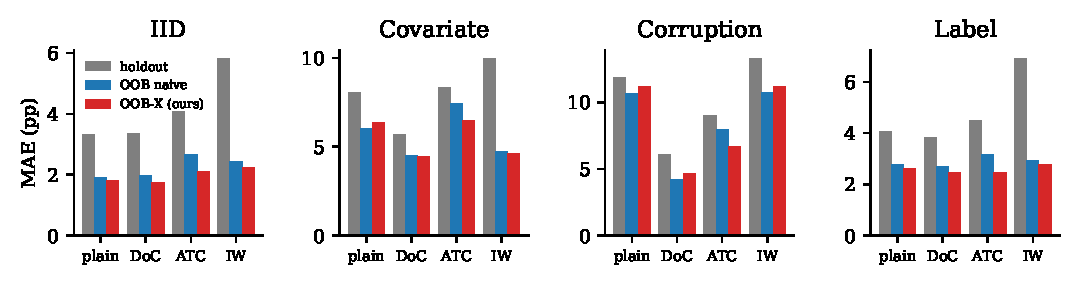
\includegraphics[width=\linewidth]{figs/main_bars.pdf}
\caption{MAE by estimator family and shift type on the main benchmark. In every panel and every family, both OOB routes (blue, red) improve on the holdout route (grey).}
\label{fig:bars}
\end{figure}

\begin{table}[t]
\centering\small
\caption{Planned paired comparisons of holdout (HO-$\Phi$) against size-extrapolated OOB (OOB-$\Phi$-X) estimators in all six experiments. $\Delta$: relative MAE reduction. Win: fraction of tasks in which OOB-X has lower absolute error. All 24 comparisons are significant after Holm correction within each experiment (two-sided Wilcoxon signed-rank test; the largest adjusted $p$ is $0.045$, for DoC on the small real datasets; all others are $<10^{-3}$).}
\label{tab:paired}
\begin{tabular}{lrcccccccc}
\toprule
 & & \multicolumn{2}{c}{plain} & \multicolumn{2}{c}{DoC} & \multicolumn{2}{c}{ATC} & \multicolumn{2}{c}{IW}\\
\cmidrule(lr){3-4}\cmidrule(lr){5-6}\cmidrule(lr){7-8}\cmidrule(lr){9-10}
Experiment & tasks & $\Delta$ & win & $\Delta$ & win & $\Delta$ & win & $\Delta$ & win\\
\midrule
Main (synthetic) & 1680 & 17\% & .64 & 26\% & .63 & 27\% & .65 & 40\% & .72\\
Ensemble-size sweep & 600 & 9\% & .57 & 14\% & .58 & 25\% & .64 & 22\% & .66\\
Sample-size sweep & 720 & 11\% & .64 & 23\% & .62 & 26\% & .63 & 29\% & .72\\
Real datasets (small) & 420 & 17\% & .63 & 7\% & .55 & 39\% & .67 & 33\% & .68\\
OpenML-CC18 (72 datasets) & 1512 & 6\% & .59 & 5\% & .55 & 11\% & .61 & 21\% & .67\\
Extra-Trees & 280 & 10\% & .65 & 14\% & .63 & 13\% & .64 & 26\% & .68\\
\bottomrule
\end{tabular}
\end{table}

\paragraph{H2 is supported in every comparison.}
Across six experiments, four estimator families and 5{,}212 tasks, the OOB route beats the holdout route in all 24 planned comparisons, with relative MAE reductions of 5--40\%. Reductions are smaller on the 72 real OpenML datasets (5--21\%) than on synthetic data (Section~\ref{sec:openml}). The gain is largest for importance weighting (21--40\%), as the variance argument in Section~\ref{sec:method} predicts: density-ratio weights shrink the effective size of an already small holdout set. The overall best estimator on the main benchmark is OOB-DoC-X (Friedman average rank 4.85 of 13; Friedman $p<10^{-100}$), followed by naive OOB-DoC (5.11) and OOB-ATC-X (5.94). The best holdout estimator, HO-DoC, ranks fourth (6.29). OOB-DoC-X is within 2\,pp of the true accuracy in 39\% of tasks and within 5\,pp in 73\%. For HO-DoC the figures are 31\% and 62\%.

\paragraph{The advantage is largest with little data.}
At $n=200$ the OOB route reduces MAE by 33\% (DoC), 38\% (ATC) and 50\% (IW; 12.9 vs.\ 6.5\,pp). At $n=1000$ the reductions are 13\%, 12\% and 23\% (all $p<10^{-9}$). The sample-size sweep (Figure~\ref{fig:nsweep}) shows the same pattern: at $n=100$ the IW error drops from 14.1 to 8.4\,pp and the ATC error from 11.9 to 6.7\,pp, and the two routes converge by $n\approx3200$, where a 20\% holdout already holds 640 points.

\begin{figure}[t]
\centering
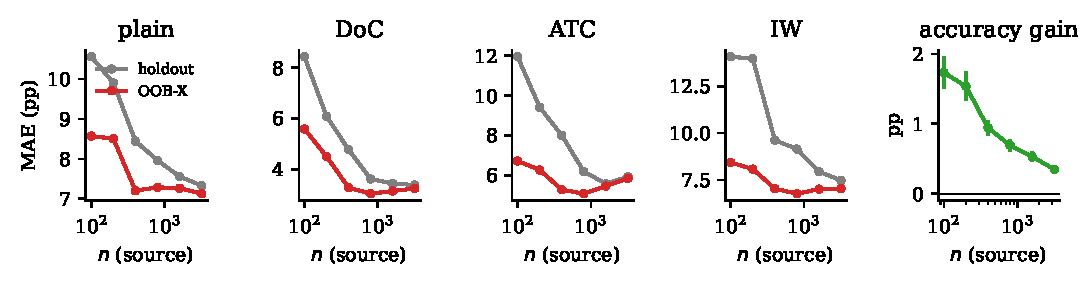
\includegraphics[width=\linewidth]{figs/nsweep.pdf}
\caption{Sample-size sweep (720 tasks; IID, covariate and corruption shift pooled). Left four panels: MAE of holdout versus OOB-X estimators. Right: target-accuracy gain of the model trained on all source data over the model trained on 80\% of it (mean $\pm$ s.e.).}
\label{fig:nsweep}
\end{figure}

\paragraph{H3 is supported: no accuracy tax.}
Because the OOB route needs no holdout, the deployed forest trains on 25\% more data. Its target accuracy is higher by 1.21\,pp on average on the main benchmark (better in 82\% of tasks, $p<10^{-170}$), by 0.96\,pp in the sample-size sweep, by 0.65\,pp for Extra-Trees and by 0.50\,pp on the real datasets. The gain decays smoothly with $n$, from 1.73\,pp at $n=100$ to 0.35\,pp at $n=3200$ (Figure~\ref{fig:nsweep}, right). The OOB route is therefore better on \emph{both} axes of the dilemma described in the introduction: a better model, and a better estimate of how good it is.

\subsection{The size mismatch and size-matched extrapolation (H1)}
\label{sec:mech}

\paragraph{Proposition~\ref{prop:oob} holds empirically.}
Figure~\ref{fig:mech}(a) compares, for 12 synthetic tasks with $T=500$, the OOB accuracy of size-$m$ sub-ensembles with the true target accuracy of size-$m$ ensembles. In-distribution, the gap is statistically indistinguishable from zero at every $m$ from 1 to 160 (means between $-0.37$ and $-0.01$\,pp, each within about one standard error). Once sizes are matched, the OOB sample is an unbiased reference sample, exactly as Proposition~\ref{prop:oob} states. Under covariate shift the gap is 2.7--7.0\,pp; this is the shift-induced change that shift-aware estimators must correct.

\paragraph{The $1/m$ law holds.}
Over the window $m\in[8,60]$, the fit $a+b/m$ explains the target-accuracy curve with median $R^2=0.992$ (IID) and $0.991$ (covariate); 96\% of the target-curve fits have $R^2>0.9$. Extrapolating from $m\le160$ to $T=500$ reduces the error with respect to the true full-ensemble accuracy from 0.54 to 0.28\,pp (Figure~\ref{fig:mech}(b,c)).

\begin{figure}[t]
\centering
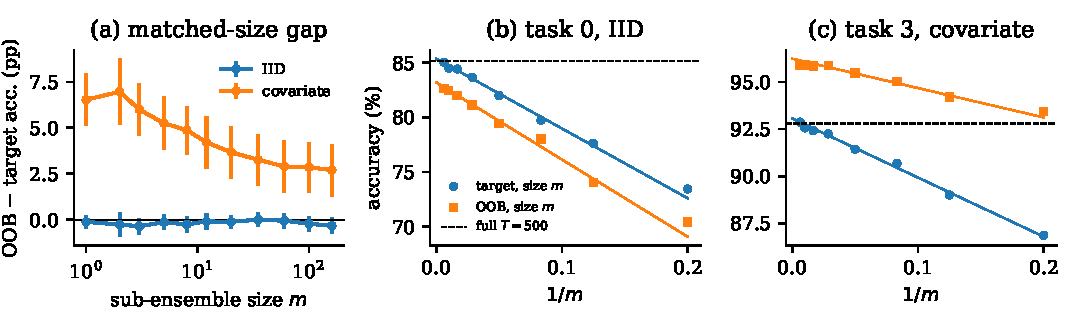
\includegraphics[width=\linewidth]{figs/mech.pdf}
\caption{Mechanism. (a) OOB accuracy minus target accuracy at matched sub-ensemble size $m$, averaged over 12 tasks (mean $\pm$ s.e.). In-distribution the gap is zero at every size (Proposition~\ref{prop:oob}). (b, c) Accuracy against $1/m$ with $a+b/m$ fits on $m\in[8,60]$. The intercept approximates the full ensemble (dashed line).}
\label{fig:mech}
\end{figure}

\paragraph{Naive OOB bias scales as $1/T$; extrapolation removes most of it.}
Figure~\ref{fig:tsweep} (top) shows the in-distribution bias as a function of $T$. The naive plug-ins are biased downwards, and the bias halves each time $T$ doubles. For the plain estimator it is $-3.98$, $-2.19$, $-1.19$, $-0.68$ and $-0.34$\,pp at $T=25,\dots,500$, as Proposition~\ref{prop:bias}(i) predicts. Size-matched extrapolation removes roughly 40--95\% of this bias. For DoC it goes from $-5.77$ to $-2.16$\,pp at $T=25$ and from $-1.50$ to $-0.19$\,pp at $T=100$; for ATC, from $-1.21$ to $-0.16$\,pp at $T=100$. The holdout estimators carry no size bias but have 1.6--3$\times$ the in-distribution MAE of the OOB-X estimators at every $T\ge100$.

\begin{figure}[t]
\centering
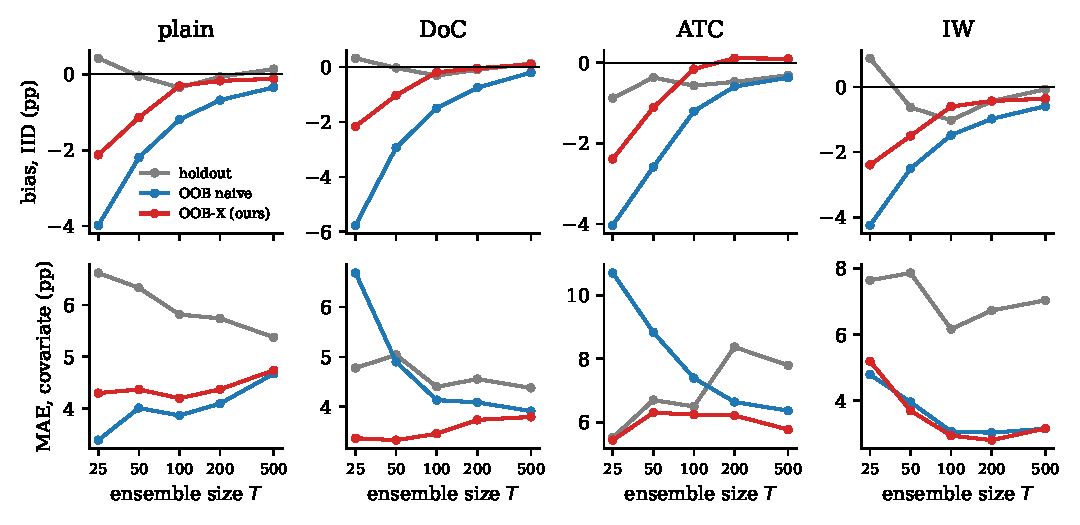
\includegraphics[width=\linewidth]{figs/tsweep.pdf}
\caption{Ensemble-size sweep (600 tasks, $n=500$). Top: signed bias in-distribution; the naive OOB bias decays as $1/T$, and extrapolation removes most of it. Bottom: MAE under covariate shift ($\alpha=2$).}
\label{fig:tsweep}
\end{figure}

\paragraph{When does extrapolation help under shift? A refinement of H1.}
Removing the size bias does not always reduce the error under shift, because the size bias can partly cancel a shift bias of the opposite sign. The outcome is consistent across experiments (Table~\ref{tab:x}).
\emph{ATC}: extrapolation reduces MAE in all six experiments (by 5--29\%, all Holm-adjusted $p<10^{-3}$). Its gains are largest under covariate shift and for small $T$; at $T=25$ under covariate shift the MAE falls from 10.7 to 5.4\,pp.
\emph{DoC}: the effect is neutral to slightly positive (MAE changes between $-4.7\%$ and $+2.1\%$; significant improvements on both real-data experiments, Extra-Trees and the ensemble-size sweep).
\emph{Plain and IW}: extrapolation removes their in-distribution bias but changes MAE by $-0.1\%$ to $+4.7\%$, because under shift these estimators already \emph{over}-estimate accuracy, and correcting the size bias moves them further upward.
We therefore recommend the extrapolated variants for ATC and DoC by default, and the extrapolated plain and IW variants only when the shift is believed to be small.

\begin{table}[t]
\centering\small
\caption{Effect of size-matched extrapolation: relative MAE change of OOB-$\Phi$-X versus naive OOB-$\Phi$ (negative values are improvements). $^{*}$: Holm-adjusted $p<0.01$ (Wilcoxon).}
\label{tab:x}
\begin{tabular}{lcccc}
\toprule
Experiment & plain & DoC & ATC & IW\\
\midrule
Main & $+4.1\%^{*}$ & $+0.7\%$ & $-15.1\%^{*}$ & $+0.7\%^{*}$\\
Ensemble-size sweep & $+4.7\%^{*}$ & $-4.5\%^{*}$ & $-29.3\%^{*}$ & $+2.9\%^{*}$\\
Sample-size sweep & $+3.3\%^{*}$ & $+2.1\%$ & $-9.5\%^{*}$ & $+1.3\%^{*}$\\
Real datasets (small) & $+2.5\%^{*}$ & $-3.0\%^{*}$ & $-7.8\%^{*}$ & $-0.0\%$\\
OpenML-CC18 & $+1.5\%^{*}$ & $-1.6\%^{*}$ & $-5.3\%^{*}$ & $+0.6\%^{*}$\\
Extra-Trees & $+4.2\%^{*}$ & $-4.7\%^{*}$ & $-13.6\%^{*}$ & $-0.1\%$\\
\bottomrule
\end{tabular}
\end{table}

\subsection{Large-scale real-data validation: OpenML-CC18}
\label{sec:openml}

The synthetic results could reflect the generator rather than real tabular data, so we repeated the full protocol on all 72 datasets of OpenML-CC18 (1{,}512 tasks; Table~\ref{tab:openml}, Figure~\ref{fig:openml}). This experiment was run after all others, and the analysis was fixed in advance.

\paragraph{The free reference set replicates, with smaller effects.}
At the task level the OOB route again beats the holdout route in all four families (Table~\ref{tab:paired}), but with smaller relative MAE reductions than on synthetic data: 6\% (plain), 5\% (DoC), 11\% (ATC) and 21\% (IW). At the more conservative \emph{dataset} level (72 paired dataset means), all four improvements remain significant after Holm correction ($p_{\mathrm{Holm}}=0.008$ for DoC, $<10^{-4}$ for the others). OOB-X is better on 54/72 datasets (plain), 45/72 (DoC), 53/72 (ATC) and 66/72 (IW). The deployed model is again more accurate, by 0.59\,pp on average, and better on 59 of the 72 datasets ($p<10^{-9}$).

\paragraph{Where the gain comes from.}
The benefit depends strongly on the shift type. It is largest in-distribution (30--47\% lower MAE in every family) and under sub-population covariate shift (9--42\%; IW falls from 5.96 to 3.48\,pp), moderate under label shift (7--17\%), and close to zero under corruption. There, plain and DoC show no significant difference ($p_{\mathrm{Holm}}=1.0$) and ATC and IW improve by only 6\%. This is expected: once corruption moves the target outside the source support, the error is dominated by the estimator's modelling assumption rather than by reference-set variance, and a larger reference set cannot fix the wrong assumption. The gain also shrinks with dataset size. For datasets with source size $n<700$, MAE falls by 12--25\%; for datasets at the 2{,}000-point cap, by 2--15\%. The improvement for DoC is not significant on medium and large datasets ($p=0.10$ and $0.06$).

\paragraph{Extrapolation.}
The pattern of Table~\ref{tab:x} replicates: extrapolation improves ATC (5.3\% lower MAE, better on 56/72 datasets) and DoC (1.6\%, 45/72), and slightly worsens plain (1.5\%) and IW (0.6\%) estimators.

\paragraph{Shift-type ranking on real data.}
OOB-IW-X is the best estimator under covariate shift (3.48\,pp) and OOB-DoC-X under corruption (10.44\,pp), while ATC fails badly under real-data corruption (at least 18.9\,pp in every variant): its threshold transfers poorly when confidences collapse. The best overall Friedman ranks belong to OOB-IW (5.80), OOB-DoC-X and OOB-IW-X (both 5.82), against 6.41 for the best holdout estimator (HO-DoC).

\begin{table}[t]
\centering\small
\caption{OpenML-CC18 (72 real datasets, 1{,}512 tasks, $T=200$): MAE in pp (mean $\pm$ s.e.).}
\label{tab:openml}
\begin{tabular}{lccccc}
\toprule
Estimator & IID & Covariate & Corruption & Label & All\\
\midrule
AC & 9.62\,\scriptsize{$\pm$0.68} & 11.02\,\scriptsize{$\pm$0.40} & 15.45\,\scriptsize{$\pm$0.64} & 12.21\,\scriptsize{$\pm$0.73} & 12.26\,\scriptsize{$\pm$0.29} \\
HO & 2.04\,\scriptsize{$\pm$0.15} & 6.96\,\scriptsize{$\pm$0.26} & 12.70\,\scriptsize{$\pm$0.59} & 6.41\,\scriptsize{$\pm$0.64} & 7.82\,\scriptsize{$\pm$0.24} \\
HO\mbox{-}DoC & 1.83\,\scriptsize{$\pm$0.14} & 4.19\,\scriptsize{$\pm$0.16} & 10.52\,\scriptsize{$\pm$0.40} & 4.92\,\scriptsize{$\pm$0.50} & 5.77\,\scriptsize{$\pm$0.17} \\
HO\mbox{-}ATC & 2.48\,\scriptsize{$\pm$0.17} & 5.96\,\scriptsize{$\pm$0.27} & 20.14\,\scriptsize{$\pm$0.86} & 4.40\,\scriptsize{$\pm$0.38} & 9.29\,\scriptsize{$\pm$0.33} \\
HO\mbox{-}IW & 2.61\,\scriptsize{$\pm$0.20} & 5.96\,\scriptsize{$\pm$0.25} & 13.86\,\scriptsize{$\pm$0.59} & 6.04\,\scriptsize{$\pm$0.56} & 7.75\,\scriptsize{$\pm$0.24} \\
OOB & 1.37\,\scriptsize{$\pm$0.10} & 6.10\,\scriptsize{$\pm$0.24} & 12.43\,\scriptsize{$\pm$0.60} & 5.93\,\scriptsize{$\pm$0.63} & 7.21\,\scriptsize{$\pm$0.24} \\
OOB\mbox{-}DoC & 1.38\,\scriptsize{$\pm$0.11} & 3.96\,\scriptsize{$\pm$0.15} & 10.48\,\scriptsize{$\pm$0.40} & 4.59\,\scriptsize{$\pm$0.50} & 5.55\,\scriptsize{$\pm$0.17} \\
OOB\mbox{-}ATC & 2.01\,\scriptsize{$\pm$0.15} & 5.11\,\scriptsize{$\pm$0.22} & 19.68\,\scriptsize{$\pm$0.81} & 4.10\,\scriptsize{$\pm$0.42} & 8.69\,\scriptsize{$\pm$0.32} \\
OOB\mbox{-}IW & 1.47\,\scriptsize{$\pm$0.12} & 3.52\,\scriptsize{$\pm$0.17} & 12.79\,\scriptsize{$\pm$0.57} & 5.00\,\scriptsize{$\pm$0.52} & 6.09\,\scriptsize{$\pm$0.22} \\
OOB\mbox{-}X & 1.30\,\scriptsize{$\pm$0.10} & 6.22\,\scriptsize{$\pm$0.24} & 12.68\,\scriptsize{$\pm$0.60} & 5.93\,\scriptsize{$\pm$0.63} & 7.32\,\scriptsize{$\pm$0.24} \\
OOB\mbox{-}DoC\mbox{-}X & \textbf{1.27\,\scriptsize{$\pm$0.09}} & 3.84\,\scriptsize{$\pm$0.15} & \textbf{10.44\,\scriptsize{$\pm$0.40}} & 4.53\,\scriptsize{$\pm$0.50} & \textbf{5.46\,\scriptsize{$\pm$0.17}} \\
OOB\mbox{-}ATC\mbox{-}X & 1.65\,\scriptsize{$\pm$0.12} & 4.77\,\scriptsize{$\pm$0.21} & 18.90\,\scriptsize{$\pm$0.80} & \textbf{3.86\,\scriptsize{$\pm$0.42}} & 8.23\,\scriptsize{$\pm$0.31} \\
OOB\mbox{-}IW\mbox{-}X & 1.37\,\scriptsize{$\pm$0.10} & \textbf{3.48\,\scriptsize{$\pm$0.17}} & 13.02\,\scriptsize{$\pm$0.57} & 5.01\,\scriptsize{$\pm$0.52} & 6.12\,\scriptsize{$\pm$0.23} \\
\bottomrule
\end{tabular}
\end{table}

\begin{figure}[t]
\centering
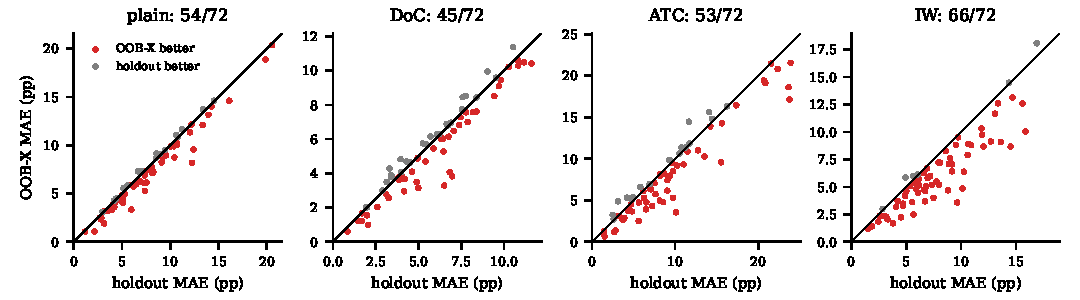
\includegraphics[width=\linewidth]{figs/openml_scatter.pdf}
\caption{OpenML-CC18, one point per dataset: mean absolute error of the holdout estimator (x) against the size-extrapolated OOB estimator (y). Points below the diagonal (red) are datasets where the free reference set is better; titles give the count out of 72.}
\label{fig:openml}
\end{figure}

\subsection{Shift-type dependence (H4)}

H4 is only \emph{partly} supported. Under corruption, which is a support shift, confidence-based estimators dominate on synthetic data, as hypothesized: OOB-DoC reaches 4.2\,pp while every IW variant is at or above 10.7\,pp, because importance weighting cannot extrapolate beyond the source support. Under sub-population covariate shift, however, IW does \emph{not} dominate on synthetic data: OOB-IW-X (4.61\,pp) and OOB-DoC-X (4.48\,pp) are statistically tied. On the three small real datasets the ordering changes: IW and plain OOB are best overall (OOB-IW-X 4.46\,pp), ATC-X is best under covariate shift (3.79\,pp), and every method fails under the strong real-data corruption (all $\ge7.8$\,pp). Label shift of the strength we used produced small accuracy changes, and all OOB-X estimators stayed within 2.8\,pp on average. In short, no estimator family is uniformly best. On synthetic data the benefit of the free reference set holds within every family and every shift type (Figure~\ref{fig:bars}); on OpenML it holds in every family but disappears for plain and DoC estimators under corruption (Section~\ref{sec:openml}).

\subsection{Small real datasets and Extra-Trees (H5)}

On the three small scikit-learn datasets (Table~\ref{tab:real}) the best estimator is an OOB variant in every column, and OOB-IW-X attains the lowest overall MAE (4.46\,pp, versus 5.59\,pp for the best holdout estimator). Per dataset, the best OOB-X estimator improves on the best holdout estimator for Breast Cancer (2.38 vs.\ 3.30\,pp), Digits (4.78 vs.\ 6.31) and Wine (4.18 vs.\ 5.75).
For bootstrapped Extra-Trees \citep{geurts2006et}, all four OOB-X estimators again beat their holdout counterparts (10--26\% lower MAE, all Holm $p<10^{-3}$; Table~\ref{tab:paired}), and the extrapolation pattern of Table~\ref{tab:x} repeats. H5 is supported.

\begin{table}[t]
\centering\small
\caption{Real datasets (Breast Cancer, Digits, Wine; 420 tasks, $T=200$): MAE in pp (mean $\pm$ s.e.).}
\label{tab:real}
\begin{tabular}{lccccc}
\toprule
Estimator & IID & Covariate & Corruption & Label & All\\
\midrule
AC & 12.06\,\scriptsize{$\pm$1.12} & 16.23\,\scriptsize{$\pm$0.72} & 22.56\,\scriptsize{$\pm$1.30} & 12.29\,\scriptsize{$\pm$1.07} & 16.88\,\scriptsize{$\pm$0.56} \\
HO & 2.82\,\scriptsize{$\pm$0.37} & 5.35\,\scriptsize{$\pm$0.43} & 8.88\,\scriptsize{$\pm$0.61} & 2.47\,\scriptsize{$\pm$0.26} & 5.59\,\scriptsize{$\pm$0.28} \\
HO\mbox{-}DoC & 2.87\,\scriptsize{$\pm$0.41} & 6.03\,\scriptsize{$\pm$0.34} & 10.56\,\scriptsize{$\pm$0.55} & 2.15\,\scriptsize{$\pm$0.24} & 6.32\,\scriptsize{$\pm$0.27} \\
HO\mbox{-}ATC & 3.05\,\scriptsize{$\pm$0.55} & 7.38\,\scriptsize{$\pm$0.75} & 14.75\,\scriptsize{$\pm$1.05} & 3.04\,\scriptsize{$\pm$0.51} & 8.25\,\scriptsize{$\pm$0.50} \\
HO\mbox{-}IW & 2.82\,\scriptsize{$\pm$0.43} & 7.57\,\scriptsize{$\pm$0.82} & 9.37\,\scriptsize{$\pm$0.64} & 2.42\,\scriptsize{$\pm$0.28} & 6.67\,\scriptsize{$\pm$0.42} \\
OOB & 1.47\,\scriptsize{$\pm$0.17} & 3.89\,\scriptsize{$\pm$0.39} & 8.52\,\scriptsize{$\pm$0.62} & 1.45\,\scriptsize{$\pm$0.14} & 4.52\,\scriptsize{$\pm$0.28} \\
OOB\mbox{-}DoC & 1.47\,\scriptsize{$\pm$0.16} & 5.79\,\scriptsize{$\pm$0.29} & 10.99\,\scriptsize{$\pm$0.62} & 1.59\,\scriptsize{$\pm$0.14} & 6.06\,\scriptsize{$\pm$0.28} \\
OOB\mbox{-}ATC & 1.52\,\scriptsize{$\pm$0.19} & 4.19\,\scriptsize{$\pm$0.42} & 11.39\,\scriptsize{$\pm$0.81} & 1.60\,\scriptsize{$\pm$0.21} & 5.50\,\scriptsize{$\pm$0.35} \\
OOB\mbox{-}IW & 1.51\,\scriptsize{$\pm$0.19} & 4.28\,\scriptsize{$\pm$0.39} & \textbf{7.76\,\scriptsize{$\pm$0.64}} & 1.34\,\scriptsize{$\pm$0.12} & 4.46\,\scriptsize{$\pm$0.28} \\
OOB\mbox{-}X & 1.50\,\scriptsize{$\pm$0.16} & 4.01\,\scriptsize{$\pm$0.40} & 8.74\,\scriptsize{$\pm$0.63} & 1.42\,\scriptsize{$\pm$0.14} & 4.63\,\scriptsize{$\pm$0.28} \\
OOB\mbox{-}DoC\mbox{-}X & \textbf{1.40\,\scriptsize{$\pm$0.14}} & 5.58\,\scriptsize{$\pm$0.28} & 10.80\,\scriptsize{$\pm$0.61} & 1.42\,\scriptsize{$\pm$0.14} & 5.88\,\scriptsize{$\pm$0.28} \\
OOB\mbox{-}ATC\mbox{-}X & 1.54\,\scriptsize{$\pm$0.19} & \textbf{3.79\,\scriptsize{$\pm$0.41}} & 10.56\,\scriptsize{$\pm$0.76} & 1.45\,\scriptsize{$\pm$0.17} & 5.07\,\scriptsize{$\pm$0.33} \\
OOB\mbox{-}IW\mbox{-}X & 1.53\,\scriptsize{$\pm$0.18} & 4.22\,\scriptsize{$\pm$0.40} & 7.84\,\scriptsize{$\pm$0.63} & \textbf{1.32\,\scriptsize{$\pm$0.13}} & \textbf{4.46\,\scriptsize{$\pm$0.28}} \\
\bottomrule
\end{tabular}
\end{table}

\subsection{Use case: detecting harmful shift}

Practitioners often need to decide whether a shift has \emph{hurt} the model, not just to estimate its accuracy. For each main-benchmark task with a shift, we computed the estimated accuracy drop relative to the IID task of the same family, sample size and seed. We then measured how well it ranks the true drop and how well it detects drops larger than 5\,pp (prevalence 47\%). OOB-ATC-X detects harmful shifts with AUROC 0.908, against 0.809 for HO-ATC, and attains a Spearman correlation of 0.80 with the true drop (HO-ATC: 0.62). OOB-DoC-X also improves on HO-DoC (AUROC 0.79 vs.\ 0.70). Plain and IW estimators are nearly blind to corruption-induced drops (AUROC $\le0.57$), which reinforces that IW should not be used to monitor support shifts.

\emph{This advantage largely does not replicate on real data.} On OpenML-CC18 (prevalence of drops above 5\,pp: 42\%), OOB-ATC-X and HO-ATC detect harmful shift almost equally well (AUROC 0.832 vs.\ 0.824; Spearman 0.66 vs.\ 0.63), and OOB-DoC-X is marginally worse than HO-DoC (0.792 vs.\ 0.799). The large synthetic gap should therefore not be relied on in practice. The robust conclusion is that ATC- and DoC-type estimators, from either reference set, detect harmful real shifts with AUROC around 0.8, whereas plain and IW estimators do not ($\le0.65$).

\subsection{Hypothesis scorecard}
\begin{center}\small
\begin{tabular}{lp{11.5cm}}
\toprule
H1 & \emph{Refined.} The bias exists and decays as $1/T$, but it is driven mainly by the accuracy mismatch rather than the confidence mismatch, so size matching alone is insufficient. Matching plus $1/m$ extrapolation removes roughly 40--95\% of it. Under shift it reliably helps ATC, is neutral for DoC, and slightly hurts plain and IW estimators.\\
H2 & \emph{Supported} in 24/24 comparisons, including at the dataset level on 72 OpenML datasets. Effects are largest at small $n$ and smaller on real data (5--21\%) than on synthetic data, and vanish for plain and DoC estimators under real-data corruption.\\
H3 & \emph{Supported}: +0.35 to +1.73\,pp target accuracy, decaying with $n$; on OpenML, +0.59\,pp, and better on 59/72 datasets.\\
H4 & \emph{Partly refuted.} Confidence methods win under synthetic corruption, but IW does not dominate under covariate shift, and rankings differ between synthetic and real data. On OpenML, IW is best under covariate shift and DoC under corruption, as hypothesized, but ATC fails under real corruption.\\
H5 & \emph{Supported} for bootstrapped Extra-Trees.\\
\bottomrule
\end{tabular}
\end{center}

\section{Discussion}
\label{sec:discussion}

\paragraph{Practical recommendations.}
For practitioners who deploy bagged tree ensembles and must monitor them without labels, the results support three rules:
(1) do not carve out a holdout reference set; use OOB predictions instead;
(2) use OOB-DoC-X as a general default and OOB-IW when the shift is believed to keep the source support, where it was the most accurate estimator on real data; avoid ATC when target corruption is possible, since it failed badly under real-data corruption;
(3) never use raw average confidence. Random forests are strongly under-confident \citep{niculescu2005probs}, and AC underestimated accuracy, on average by 4.5--23\,pp, in every experiment and shift type.
The method needs no additional model fitting except the domain classifier for IW. For $n=1000$, $n_Q=2000$ and $T=200$ on a single CPU core, our unoptimized implementation computes all naive and extrapolated confidence-based estimators in 0.76\,s, compared with 0.41\,s to fit the forest; the IW domain classifier adds 1.4\,s.

\paragraph{Why the free reference set wins.}
Two effects act together. The reference set is five times larger, which reduces the variance of every reference-set statistic. It is most important for IW, whose effective sample size is further reduced by the weights. Meanwhile the deployed model is better, which matters most at small $n$. Proposition~\ref{prop:oob} and Figure~\ref{fig:mech}(a) show that the price, a model mismatch, is entirely an ensemble-size effect. That effect is predictable and correctable.

\paragraph{Relation to disagreement-based estimation.}
Disagreement-based estimators \citep{jiang2022gde,baek2022aotl} also exploit the randomness of training, but they require independently trained models and calibration assumptions on the ensemble. Our approach is complementary: it uses the bagging randomness to obtain held-out \emph{labels} for free and leaves the choice of estimator open. Combining OOB reference sets with agreement-on-the-line style estimators is a natural next step.

\paragraph{Limitations.}
We state the limitations plainly.
\emph{(i) Real-data scale.} The real-data evaluation covers the 72 datasets of OpenML-CC18 with 3 seeds each and source samples capped at 2{,}000 points. Larger datasets, where a 20\% holdout is already big, would likely show smaller gains, consistent with the size trend in Section~\ref{sec:openml}.
\emph{(ii) Shift realism.} The shifts are controlled and synthetic: PCA-based sub-population selection, Gaussian corruption, and Dirichlet label shift. Natural temporal and geographic shifts, as in Folktables \citep{ding2021folktables}, may behave differently.
\emph{(iii) Scope of models.} The method applies only to bagged ensembles; boosting does not produce OOB predictions of the same kind. Bagged neural networks or bagged gradient boosting would fall within scope but were not evaluated.
\emph{(iv) Extrapolation under shift.} Correcting the size bias is not always beneficial for plain and IW estimators under shift (Table~\ref{tab:x}). The $1/m$ law is an assumption that we verified empirically, not a theorem for all estimator families.
\emph{(v) Concept shift.} Like all label-free methods, ours cannot detect changes in $p(y\mid x)$ that leave the covariates and confidences unchanged.
\emph{(vi) Metrics.} We studied accuracy only; extensions to AUROC and F1, as in PAPE \citep{bialek2025pape}, are straightforward, since any reference-set estimator can be fed OOB scores.

\section{Conclusion}
\label{sec:conclusion}

Label-free performance estimation under distribution shift has relied on labeled reference sets that cost training data. For bagged ensembles this cost is unnecessary: the out-of-bag sample is an exact held-out reference sample, but for a smaller ensemble. Once this size mismatch is understood, it can be corrected with size-matched, $1/m$-extrapolated estimators. In a pre-registered study of 5{,}212 tasks, including all 72 datasets of OpenML-CC18, the free reference set reduced estimation error in every estimator family and every experiment, by 5--21\% on real data and up to 40\% on synthetic data, while also yielding a more accurate deployed model. The gains are largest for small datasets, which is exactly where carving out a holdout set hurts most, and smallest under corruption shift, where the estimators' own assumptions, not the reference set, limit accuracy. Since random forests remain among the most widely deployed models for tabular data, this is a zero-cost improvement to how such models can be monitored in the field.

\paragraph{Reproducibility.}
All code (estimators, shift generators, experiment runners, analysis and figure scripts), the pre-registered hypotheses and all raw per-task results are provided as supplementary material and will be released publicly upon publication. Every number in this paper is produced by the released analysis scripts.

\paragraph{Declaration of generative AI and AI-assisted technologies in the manuscript preparation process.}
During the preparation of this work the author used Claude Sonnet 5 to edit the manuscript to improve readability. After using this tool/service, the author reviewed and edited the content as needed and take full responsibility for the content of the published article.


\bibliographystyle{plainnat}
\bibliography{refs}
\appendix
\section{Implementation details}
\label{app:impl}
\paragraph{Forests.} scikit-learn~1.9 \texttt{RandomForestClassifier} and \texttt{ExtraTreesClassifier(bootstrap=True)} with default hyperparameters (fully grown trees, $\sqrt d$ candidate features per split, Gini impurity). OOB membership is read from \texttt{estimators\_samples\_}.
\paragraph{Domain classifier.} A random forest with 200 trees and \texttt{min\_samples\_leaf}$=5$, trained to separate source ($0$) from target ($1$) covariates; source-point probabilities are its OOB probabilities, clipped to $[10^{-3},1-10^{-3}]$; weights are clipped at 20 and normalized to mean one. The same procedure is used for HO-IW on the holdout reference set.
\paragraph{Extrapolation.} $m_{\max}$ is the 10th percentile of OOB counts, so that 90\% of source points contribute at every grid size; the grid contains $G=5$ integers equally spaced in $[m_{\max}/4,m_{\max}]$ (duplicates removed); $R=8$ repetitions; jitter $\epsilon\sim U(0,10^{-7})$. Final estimates are clipped to $[0,1]$.
\paragraph{Synthetic task families.} Family $c\in\{0,\dots,39\}$ draws its generator parameters from a random generator seeded with $1000+c$: $d\sim U\{10,\dots,40\}$, $K\sim U\{2,\dots,5\}$, informative features $\max(\lceil\log_2 2K\rceil+1,\lfloor u d\rfloor)$ with $u\sim U(0.2,0.6)$, redundant features $\sim U\{0,\dots,\lfloor(d-\text{inf})/2\rfloor-1\}$, clusters per class $\sim U\{1,2\}$, class separation $\sim U(0.6,1.6)$, label-flip rate $\sim U(0,0.08)$.
\paragraph{Compute.} The 3{,}700 synthetic and small-real-data tasks ran on two CPU cores in about three hours of wall-clock time; the 1{,}512 OpenML-CC18 tasks ran on a two-core Google Colab instance in about four hours.

\section{Additional results}
\begin{table}[h]
\centering\small
\caption{Main benchmark MAE (pp) by shift condition and severity.}
\label{tab:levels}
\begin{tabular}{lccccccc}
\toprule
Estimator & IID & Cov.\,$\alpha{=}1$ & Cov.\,$\alpha{=}2$ & Cov.\,$\alpha{=}3$ & Corr.\,$s{=}0.5$ & Corr.\,$s{=}1$ & Label \\
\midrule
HO & 3.32 & 4.68 & 7.44 & 12.14 & 7.29 & 16.46 & 4.07 \\
HO\mbox{-}DoC & 3.37 & 4.00 & 5.06 & 8.06 & 4.75 & 7.38 & 3.82 \\
HO\mbox{-}ATC & 4.08 & 5.36 & 8.09 & 11.54 & 6.50 & 11.51 & 4.48 \\
HO\mbox{-}IW & 5.82 & 6.90 & 9.70 & 13.29 & 8.56 & 18.00 & 6.91 \\
OOB\mbox{-}X & 1.80 & 2.99 & 5.88 & 10.25 & 5.74 & 16.63 & 2.63 \\
OOB\mbox{-}DoC\mbox{-}X & \textbf{1.74} & \textbf{2.72} & 4.39 & \textbf{6.34} & \textbf{2.80} & \textbf{6.48} & \textbf{2.45} \\
OOB\mbox{-}ATC\mbox{-}X & 2.11 & 3.14 & 6.32 & 9.95 & 4.33 & 9.09 & 2.48 \\
OOB\mbox{-}IW\mbox{-}X & 2.24 & 3.20 & \textbf{4.28} & 6.36 & 5.52 & 16.79 & 2.79 \\
\bottomrule
\end{tabular}
\end{table}

\end{document}
